\documentclass{article}
\usepackage{geometry}
\usepackage{natbib}
\usepackage{amssymb}
\usepackage{amsmath}
\usepackage{graphicx}
\usepackage{hyperref}
\usepackage{textcomp}

\geometry{
	a4paper,
	total={170mm,257mm},
	left=30mm,
	top=30mm,
	bottom=20mm,
	right=20mm
}
\title{
	Projeto de Iniciação Científica - Relatório 1\\
	Visualização Unidimensional do Espaço Tridimensional \\
	\large Prólogo para Visualização Bidimensional do Espaço Quadridimensional
}
\date{2023-06-28}
\author{Paulo Roberto Rodrigues da Silva Filho\\ \small Felipe Acker (Orientador)}

\newcommand\R{\mathbb{R}}

\begin{document}
	\renewcommand{\figurename}{Figura}
	\graphicspath{ {./imagens/} }
	\maketitle
	\tableofcontents
	
	\section{Introdução}
	
	\paragraph{}
	Atualmente, os algoritmos de Ray-Tracing, visualização e radiosidade, para projeção de espaços 3D em 2D estão dominados e tecnologicamente avançados, já tendo mesmo implementações em Hadware, através de placas de vídeo 3D \textit{\textbf{[adicionar referências]}}. Entretanto, tais técnicas implementam a representação do espaço tridimensional no espaço bidimensional, reduzindo apenas uma dimensão de representação, e apenas para o caso particular de $\R^3$. Entratanto, não há tecnologias consistentes que permitam a redução de $\R^3$ para $\R$, ou de $\R^4$ para $\R^2$ - objetivo final desse projeto.
	
	\paragraph{}
	Assim, foi necessário desenvolver a tecnologia e os algoritmos para essas representações da estaca zero. Esse relatório visa apresentar os cálculos necessários para prover tal renderização de objetos tridimensionais, em projeção unidimensional, utilizando o modelamento físico de olho, apresentado na proposta e na renderização de objetos quadridimensionais em projeção bidimensional.
	
	\paragraph{}
	O processo de irradiação luminosa e focalização é estendido do caso tridimensional para o caso quadridimensional, enquanto o processo de captura de imagem é reduzido do caso bidimensional para o caso unidimensional, nas projeções de $\R^3$ para $\R$, ou do caso tridimensional para o caso bidimensional, nas projeções de $\R^4$ para $\R^2$.
	
	\paragraph{}
	Em um primeiro momento, é entendido o processo de renderização de objetos bidimensionais em uma tela monodimensional, com a utilização de sombras, com o cálculo de radiosidade, mas sem a utilização completa de \textit{ray-tracing}, ou seja, não serão consideradas superfícies espelhadas. A partir daí, esse algoritmo é estendido para a renderização de objetos tridimensionais em tela monodimensional - que é o objetivo planejado para esse projeto - e, por último, esse algoritmo é estendido para a renderização de objetos quadridimensionais em telas bidimensionals, o que já seria o objetivo final do projeto. 
	
	\section{Modelo Mínimo - Ambiente Bidimensional em Tela Monodimensional}
	
	\paragraph{}
	O modelo mínimo é a renderização de objetos bidimensionais em uma tela unidimensional. Esse modelo de renderização é \textbf{inferior} ao que já é implementado atualmente em software e em hardware, pelas placas 3D, mas é a base do modelo de renderização quadridimensional - portanto, entendê-lo é fundamental para a implementação de modelos de renderização que fujam do padronizado, que é a Renderização de Ambientes Tridimensionais em Telas Bidimensionais.
	
	\paragraph{}
	Para haver renderização, é necessário haver \textbf{iluminação} e \textbf{captura}. A captura é feita pelo olho, é já é uma característica da renderização assumida por definição. A iluminação, apesar de obrigatória para a renderização, não é imediatamente considerada pelo senso comum. Entretanto, renderização sem um modelo de iluminação adequada apresentaria figuras achatadas e sem volume aparente, que permitiria discernir sobre as formas representadas na renderização.
	
	\paragraph{}
	Usamos dois modelos de iluminação: \textbf{(1)} Iluminação Paralela, adequada para ambientes externos e \textbf{(2)} Iluminação radial, adequada para ambientes internos. Em ambos os casos adicionamos um componente de iluminação difusa. Não é apresentado o algoritmo de \textit{tinting}, então todas as fontes luminosas são brancas e não é apresentado o algoritmo para a utilização de mais de uma fonte luminosa. Essas omissões são corrigidas posteriormente, em uma seção específica para elas.
	
	\subsection{Iluminação Paralela}
	
	\paragraph{}
	Na iluminação paralela de ambiente bidimensional, a fonte de luz é representada como uma reta que emite luz na direção perpendicular de sua linha - ou seja, nas suas normais, em todos os pontos. A estrutura de visualização possui seus elementos apresentandos nas Figuras \ref{fig:rend} e \ref{fig:radio}. A iluminação paralela assume que não há decaimento de intensidade, mas esse modelo não é necessariamente verdadeiro em todos os cenários. Para um melhor entendimento do modelamento da intensidade luminosa, a seção a seguir, \ref{intensidade}, apresenta o racional físico/geométrico da intensidade, e um modelo extendido de como lidar com a intensidade luminosa.
	
	\subsubsection{Modelamento de Intensidade de Iluminação} \label{intensidade}
	
	\paragraph{}
	A intensidade luminosa é parte integrante do cálculo da radiosidade. No nosso mundo real (que é um mundo tridimensional), a intensidade luminosa representa a dispersão da \textbf{energia} dispersada por uma fonte de luz, no tempo (ou seja, é uma medida de potência), por uma superfície. A unidade de intensidade luminosa é a \textbf{Candela}. \textit{\textbf{[adicionar referências]}}. 
	
	\paragraph{}
	Uma das características fundamentais do decaimento luminoso, em função da distância, é que se assume que a luz se dispersa pelo ângulo sólido no qual ela se propaga a partir de sua fonte central. Assim, de uma fonte de luz paralela, não haveria decaimento de intensidade, nem de fonte de luz coerente (como no caso dos \textit{lasers}), mas em focos de luz ordinários, o decaimento seria com o quadrado da distância, pois essa é a área da superfície do ângulo sólido, na medida em que nos distanciamos do centro de emissão da luz.
	
	\paragraph{}
	Para a renderização de imagens, a intensidade máxima de iluminação representa que nenhuma das cores da linha, superfície ou variedade iluminada possui qualquer tipo de desconto de brilho, por conta da distância da fonte de luz. \textbf{Continua...}
	
	
	\paragraph{}
		\begin{figure}[h]
		\centering
		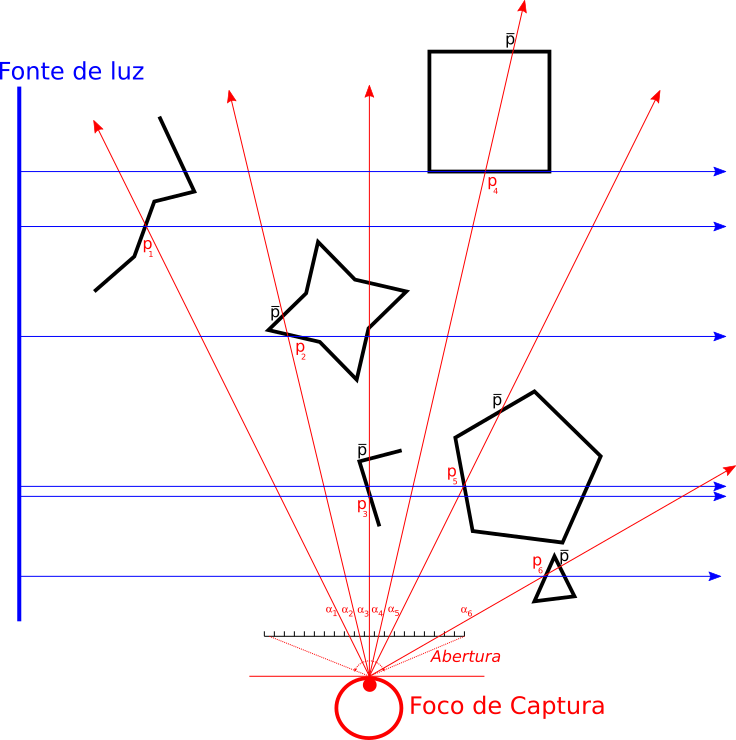
\includegraphics[scale=0.8]{Renderizacao-2D-1D}
		\caption{Identificando pontos de renderização.}
		\label{fig:rend}
	\end{figure}
	
	\paragraph{}
	\begin{figure}[h]
		\centering
		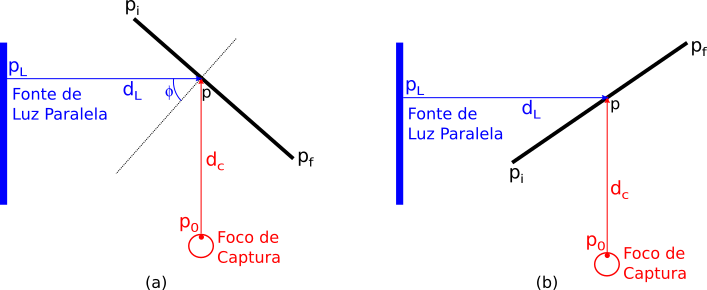
\includegraphics[scale=0.7]{radiosity}
		\caption{Identificando pontos de renderização.}
		\label{fig:radio}
	\end{figure}

	\paragraph{}
	\textbf{Continua...}

	\subsection{Iluminação Radial}
	
	\paragraph{}
	\begin{figure}[h]
		\centering
		\includegraphics[scale=0.8]{Renderizacao-2D-1D-radial}
		\caption{Identificando pontos de renderização.}
		\label{fig:rend-rad}
	\end{figure}
	
	\paragraph{}
	\begin{figure}[h]
		\centering
		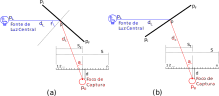
\includegraphics[scale=0.7]{radiosity-radial}
		\caption{Identificando pontos de renderização.}
		\label{fig:radio-rad}
	\end{figure}

	\paragraph{}
	\textbf{Continua...}
	
	\section{Modelo Ampliado (1) - Ambiente Tridimensional em Tela Monodimensional}
	
	\paragraph{}
	\textbf{Continua...}
	
	\section{Modelo Ampliado (2) - Ambiente Quadridimensional em Tela bidimensional}
	
	\paragraph{}
	\textbf{Continua...}
	
	\section{Modelo Ampliado (3) - Ambiente N-Dimensional em Tela M-dimensional}
	
	\paragraph{}
	\textbf{Continua...}
	
	\section{Múltiplas fontes de Luz e \textit{tinting}}
	
	\paragraph{}
	Essa seção apresenta a implementação da importante omissão do uso de múltiplas fontes de luz e do \textit{tinting}. O \textit{tinting} é a aplicação de fontes de luz coloridas, que alteram as cores dos objetos iluminados segundo regras específicas diferentes do \textit{alpha-blending} utilizado nas renderizações apresentadas acima. Já o uso de multiplas fontes de luz provoca um grande aumento de complexidade para a renderização de cada pixel da tela, ainda mais, considerando que cada fonte de luz pode ter uma cor diferente, alterando as regras de \textit{tinting}.
	
	\textbf{Continua...}
	
	\section{Conclusões e Próximos Passos}
	
	\paragraph{}
	\textbf{Continua...}

	
\end{document}